\begin{figure}[tbp]\centering
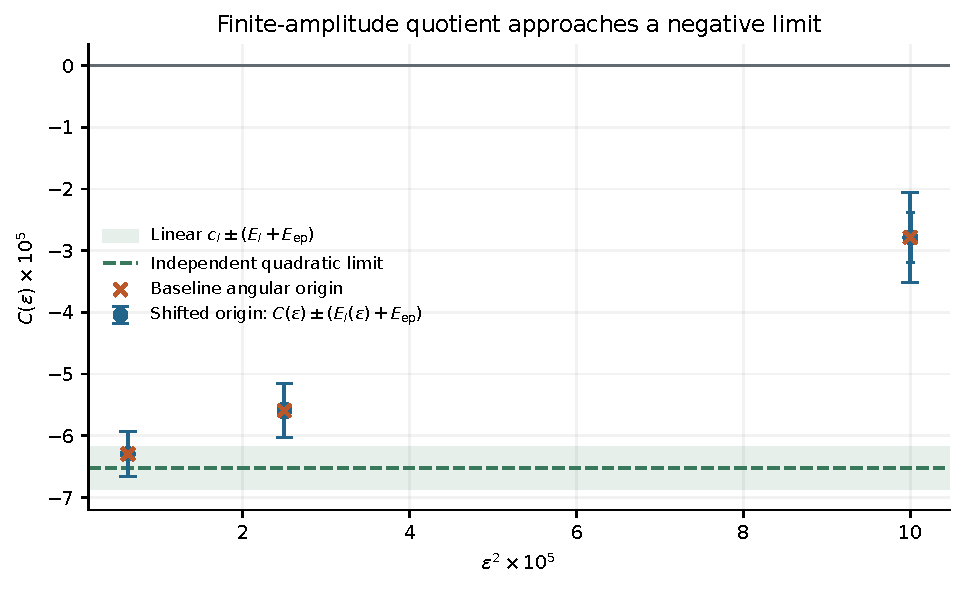
\includegraphics[width=\textwidth]{figures/fig03_nonlinear_quotient.pdf}
\caption{Paired nonlinear quotients approach the quadratic limit. Inner bars give the complete numerical allowance; outer bars add $E_{\mathrm{ep}}$ once, and the horizontal band gives the second linear coefficient and its total allowance. Baseline angular-origin values use the same physical direction and linear baseline.}\label{fig:quotient}
\end{figure}
\begin{figure}[tbp]\centering
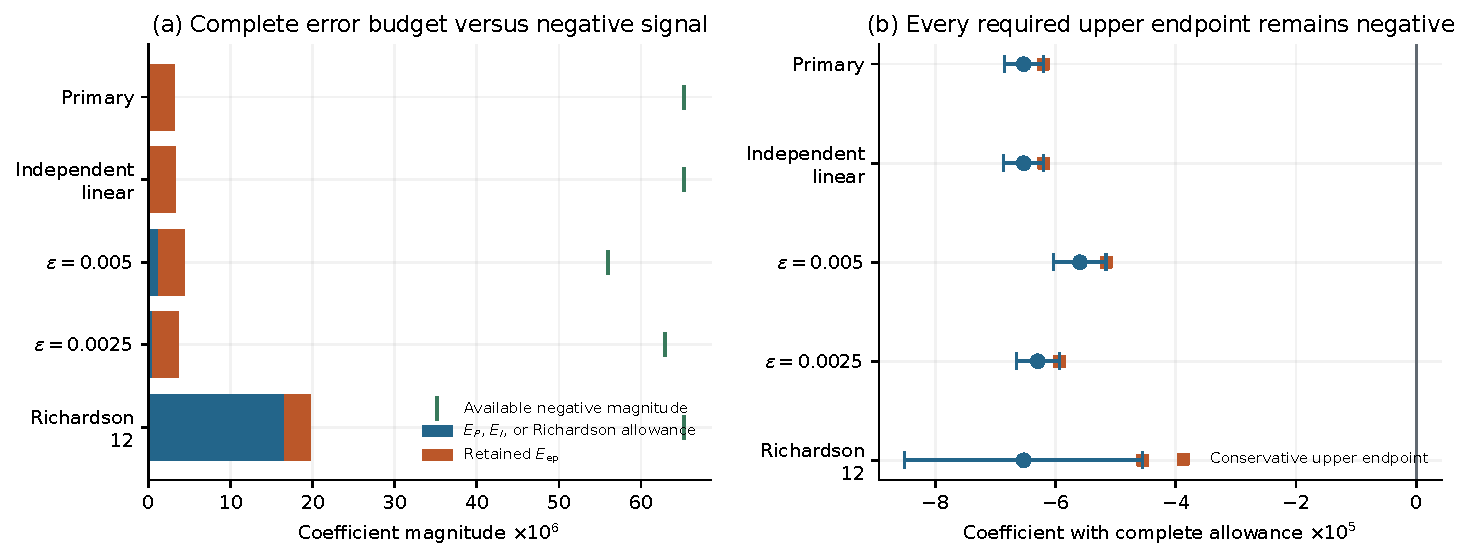
\includegraphics[width=\textwidth]{figures/fig07_error_margin.pdf}
\caption{Negative sign margins after numerical and endpoint allowances. The left panel compares coefficient magnitudes with the two allowances; the right shows centres, complete radii, and empirical upper endpoints. The Richardson value is an extrapolation diagnostic.}\label{fig:margin}
\end{figure}
\FloatBarrier
